\chapter{Fejlesztői dokumentáció} % Developer guide
\label{ch:impl}

% ==========================================================
% |                Használt technológiák                   |
% ==========================================================
\section{Használt technológiák}
Az alkalmazás fejlesztését JavaScript nyelven kezdtem meg és fejlesztés közben váltottam TypeScript nyelvre. A TypeScript gyakorlatilag egy típusos kiterjesztése a JavaScriptnek, éppen ezért minden kód amit JavaScriptben írtam azok érvényes és valid kódok TypeScriptben is. A TypeScript lényege, hogy típus biztossá teszi az alkalmazást, ami ugyan megnehezíti a fejlesztést, de nagy előnye, hogy sok probléma már a fejlesztés során észlelhető - ezáltal javítható - és nem a kész verzióban történnek katasztrofális dolgok. Váltásom motivációja a TypeScript nyújtotta előnyök mellett az is volt, hogy az ipar jelenlegi trendjei teljesen egészében effelé a nyelv felé mutatnak, minden komolyan vehető program - amely Electront, Angulart vagy más hasonló webes technológiát használ - már TypeScript nyelven íródik. Ez predesztinálta az én hozzáállásomat is a nyelvhez, tekintve a legelejétől fogva célom volt a legfrissebb és legnépszerűbb technológiák haszálata, ezen piacképes tudások elsajátítása.

Az alkalmazás fejlesztése teljes egészében a Visual Studio Code nyílt forráskódú kódszerkesztőben zajlott, Electron-t, React-et és Redux-ot továbbá Git verziókezelő rendszert használtam és egy publikus GitHub repositoryban tároltam a kódot, amely elérhető az alábbi címen: \url{https://github.com/TMD44/mvp}

\subsection{Electron}
Az Electron\footnote{\url{https://www.electronjs.org/}} egy nyílt forráskódú keretrendszer, amelyet asztali alkalmazások fejlesztéséhez lett kifejlesztve. Különlegessége, hogy a már ismert és bejáratott webes technolgiákat - tehát HTML, CSS, JavaScript - lehet használni asztali alkalmazások fejlesztéséhez. Az Electron két külön, egymástól hermetikusan elzárt része a {\it main process} és a {\it renderer process}, melyek között alá-fölé rendelt viszony található.

Az Electron ``fő szála'' - ezt nem véletlenül tettem idézőjelbe, tekintve a JavaScript egy egyszálú programozási nyelv, tehát JavaScriptben nem tudunk konkurrens programokat írni -, vagy hívhatjuk angolul {\it main process}nek is, ami gyakorlatiag egy Node.JS alkalmazás, amely a böngésző ablakok létrehozásáért, az operációs rendszerrel való kommunikációért és az alkalmazás életciklusárt felel. Ez gyakorlatilag egy fájl, amely az alkalmazásunk belépési pontját fogja képezni.

Az előbb említett böngésző ablak pedig az Electron másik elszeparált és alárendelt része, a {\it renderer process}, amelyet a {\it main process} hoz létre és menedzseli is azt. Ez tulajdonképpen egy Chromium böngésző ablakot fog jelenteni, amely egy HTML fájlt fog megjeleníteni, ahogy azt a webes világban már megszokhattuk. Lehetőgésünk van továbbá Node intergrációhoz is, amit a {\it main process}en belül tudunk engedélyezni. Az integráció lényege, hogy a böngésző ablakból használhatjuk a Node által nyújtott funckiókat is, például fájlrendszer elérése, modulok importálása és exportálása.

\subsection{React}
A React\footnote{\url{https://reactjs.org/}} egy JavaScript könyvtár, amely főleg felhasználó felületek készítésére nyújt egy fölöttébb elegáns megoldást. A segítségével rendkívül egyszerűen tudunk, úgy nevezett Single Page Application-ket készíteni. Az innováció ebben a megközelításben az, hogy nincs szükség az oldal újbóli betöltésére, hanem a felhasználói interakció során az oldal tartalmai dinamikusan újratölthetőek és nem is az egész oldal, hanem annak kisseb részei, úgy nevezett komponensei.

\subsection{Redux}
A Redux\footnote{\url{https://redux.js.org/}} egy state management tool, vagyis magyarul egy állapot kezelő rendszer. A Redux lényege és legnagyobb előnye, hogy az alkalmazásunk állapotát képes külön, egy külön egységként tárolni és menedzselni. Az állapotot memóriában tárolja, gyakorlatilag egy nagy JSON objektumban, ezen adatok módosítása pedig {\it dispatch} útján valósítható meg.

% ==========================================================
% |                 Megvalósítási terv                     |
% ==========================================================
\section{Megvalósítási terv}

\subsection{Követelmény specifikáció}
Az alkalmazás működéshez és a feladatleírás teljesítéséhez az alábbi funkciókat kell implementálni:
\begin{itemize}
    \item {\textbf {Film felsoroló platform: }} Az alkalmazásnak felületet kell biztosítania a beolvasott média tartalmak megjelenítéséhez, listázásához.
    \item {\textbf {Média tartalmak beolvasása: }} Mappák kiválasztásával az azokban fellelhető média tartalmak beolvasása.
	\item {\textbf {Keresés a média tartalmak között: }} Az alkalmazásnak lehetőséget kell bizotsítania a beolvasott média tartlamak közötti kereséshez.
	\item {\textbf {Lejátszás, Megállítás, Pörgetés: }} Bizotsítania kell a videók lejátszását.
	\item {\textbf {Felirat választás: }} Feliratok megjelenítése lejátszáskor, amennyiben elérhető.
	\item {\textbf {Sorozatok és filmek kezelése: }} A felület kezelje külön a sorozatokat és filmeket, tehát például a sorozat epizódjai ne külön-külön jelenjenek meg a listában, hanem a sorozatra rákkatintva, annak részletező ablakjában legyenek listázva az epizódok.
	\item {\textbf {Metaadatok betöltése és letölése: }} Használható és értelmes adatok beolvasása fájlnévből, mappanévből, NFO fájlból és külső adatbázisból metadatokat kell tudnia letölteni.
    \item {\textbf {Lejátszási listák: }} Lehessen lejátszási listákat létrehozni, ezen listákat filmekkel feltölteni.
\end{itemize}

\subsection{Adatok tárolása, kezelése}
Az alkalmazás futása közben a Redux segítségével kezeljük a felhasznlói felülethez és a beolvasott média tartalmakhoz kapcsolódó adatokat. Reduxot főleg webalkalmazásokhoz használnak, de nekünk itt asztali környezetben is alkalmazható lesz egy kis trükkel, mégpedig amikor megnyitjuk az alkalmazást, a Redux beállítja a kezdeti állapotot - ez a webes körnezetben annyit tenne, hogy egy előre meghatározott alapértelmezett állapot sémát alakalmazna - ami a mi esetünkben két fájl lesz, a {\it config.json} és a {\it mediaDB.json}. A {\it config.json} fájl az alkalmazás futásához, a beolvasáshoz és a felhasználó személyes preferenciáihoz szükséges adatokat, míg a {\it mediaDB.json} a beolvasott média tartalmakhoz kapcsolodó adatokat, metaadatokat tartalmazza. Ez a két JSON fájl két féleképpen jöhet létre:
\begin{itemize}
    \item Létrejöhet az alkalmazás bezárásakor, ekkor az alkalmazás jelenlegi állapota kerül kiírásra a fájlba.
    \item Valamint létrejöhet az alkalmazás indításakor is, ha a program úgy érzékeli, hogy a megadott helyen még nem létezik ez a két fájl. Ilyenkor egy előre megadott alapértelmezett állapot kerül kiírásra, amely alapértelmezett beállításokat (felhasználói felület, beolvasásssal kapcsolatos preferenciák stb.) és egy üres vázat tartalmazza, amelybe bekerülnek majd a scannelés során gyűjtött adatok.
\end{itemize}

\begin{figure}[H]
	\centering
	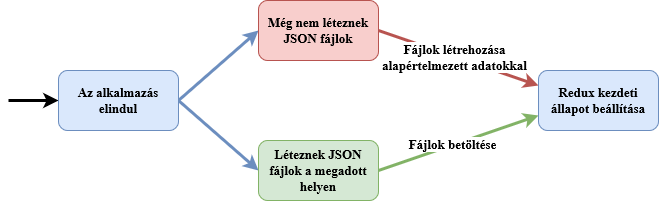
\includegraphics[width=1\textwidth]{Redux_init.png}
	\caption{A Redux kezdeti állapot beállítása}
	\label{fig:redux-init}
\end{figure}

Tehát az alkalmazás futása közben az adatok a Redux store-ban tárolódnak, amikor az alkalmazás bezárásra kerül, akkor az állapot két fájlba kerül kírásra - ebből fakadóan két futás között az adatok fájlban átrolódnak - amit aztán újranyitás esetén egyszerűen betöltünk a kezdeti állapotba

\subsubsection{Példa config.json fájl}

\lstset{caption={Példa config.json fájl}, label=src:json}
\begin{lstlisting}[language={json}]
{
"creation_time": "2021.05.10. 12:00:00",
"modification_time": "2021.05.10. 12:00:00",
"user_info": { "name": "Anonymous" },
"app_info": {
    "app_name": "Multimedia Visualization Platform",
    "app_version": "0.1.0",
    "app_current_directory": "G:\\mvp\\src\\main",
    "app_locale": "hu",
    "app_locale_country_code": "HU",
    "app_paths": {
        "home": "C:\\Users\\tmd-pc",
        "user_data": "C:\\Users\\tmd-pc\\AppData\\Roaming\\Multimedia Visualization Platform",
        "desktop": "C:\\Users\\tmd-pc\\Desktop",
        "downloads": "C:\\Users\\tmd-pc\\Downloads",
    }
},
"scan_preferences": {
    "scan_language": "en-US",
    "scan_paths": [ "G:\\SOROZATOK" ],
    "scan_file_types": {
        "media": [ ".mkv",".mp4",".avi" ],
        "sub": [ ".srt",".ass",".vtt",".ssa",".sub",".stl",".scc" ],
        "nfo": [ ".nfo" ]
    },
    "scan_results": {
        "media": [{
            "fn": "Game.of.Thrones.S01E01.BDRIP.x264.Hun.Eng",
            "ext": ".mkv",
            "path": "G:\\SOROZATOK\\Game.of.Thrones.COMPLETE.BDRIP.x264.Hun.Eng",
            "full": "G:\\SOROZATOK\\Game.of.Thrones.COMPLETE.BDRIP.x264.Hun.Eng\\Game.of.Thrones.S01E01.BDRIP.x264.Hun.Eng.mkv"
            }],
        "sub": [{
            "fn": "Game.of.Thrones.S01E01.BDRIP.x264.Hun.Eng",
            "ext": ".srt",
            "path": "G:\\SOROZATOK\\Game.of.Thrones.COMPLETE.BDRIP.x264.Hun.Eng",
            "full": "G:\\SOROZATOK\\Game.of.Thrones.COMPLETE.BDRIP.x264.Hun.Eng\\Game.of.Thrones.S01E01.BDRIP.x264.Hun.Eng.srt"
            }],
        "nfo": [{
            "fn": "Game.of.Thrones.COMPLETE.BDRIP.x264.Hun.Eng",
            "ext": ".nfo",
            "path": "G:\\SOROZATOK\\Game.of.Thrones.COMPLETE.BDRIP.x264.Hun.Eng",
            "full": "G:\\SOROZATOK\\Game.of.Thrones.COMPLETE.BDRIP.x264.Hun.Eng\\Game.of.Thrones.COMPLETE.BDRIP.x264.Hun.Eng.nfo"
            }],
    }
}}
\end{lstlisting}

\subsubsection{Példa mediaDB.json fájl}

\lstset{caption={Példa mediaDB.json fájl}, label=src:json}
\begin{lstlisting}[language={json}]
{
"creation_time": "2021.05.09. 14:44:49",
"modification_time": "2021.05.09. 14:44:49",
"movies": {
    "23b5b6d765ac7a28badbd2f6e6d31ea3": {
        "id": [ "23b5b6d765ac7a28badbd2f6e6d31ea3" ],
        "media_type": "movie"
    },
    "6209ef3cb9451c0def78013521b84d5f": {
        "id": [ "6209ef3cb9451c0def78013521b84d5f" ],
        "media_type": "movie"
    },
},
"tv_series": {
    "Game of Thrones": {
        "id": [
            "98cddc3eb8b19c7ebb2a84049c5fc4f0",
            "6a216938ea15d2a1e5282ec47d9a0649",
            "6044b7976f57147dd35da9c3719fd921",
        ],
        "media_type": "series"
    }
},
"playlists": {
    "Game of Thrones Best of": {
        "contents": {
            "Game of Thrones": {
                "id": [
                    "98cddc3eb8b19c7ebb2a84049c5fc4f0",
                    "6a216938ea15d2a1e5282ec47d9a0649",
                    "6044b7976f57147dd35da9c3719fd921",
                ],
                "media_type": "series"
            }
        },
        "media_type": "playlist"
    }
},
"all_media": {
    "98cddc3eb8b19c7ebb2a84049c5fc4f0": {
        "id": "98cddc3eb8b19c7ebb2a84049c5fc4f0",
        "media_name": "Game.of.Thrones.S01E01.BDRIP.x264.Hun.Eng",
        "extension": ".mkv",
        "path": "G:\\SOROZATOK\\Game.of.Thrones.COMPLETE.BDRIP.x264.Hun.Eng",
        "full_path": "G:\\SOROZATOK\\Game.of.Thrones.COMPLETE.BDRIP.x264.Hun.Eng\\Game.of.Thrones.S01E01.BDRIP.x264.Hun.Eng.mkv",
        "subtitles": [ "G:\\SOROZATOK\\Game.of.Thrones.COMPLETE.BDRIP.x264.Hun.Eng\\Game.of.Thrones.S01E01.BDRIP.x264.Hun.Eng.vtt" ],
        "nfo": "G:\\SOROZATOK\\Game.of.Thrones.COMPLETE.BDRIP.x264.Hun.Eng\\Game.of.Thrones.COMPLETE.BDRIP.x264.Hun.Eng.nfo",
        "metadata": {
            "title": "Game of Thrones",
            "season": 1,
            "episode": 1,
            "languages": ["HUN", "ENG"],
            "codec": "X264",
            "quality": "BDRIP",
            "media_type": "series",
            "imdb_id": "tt0944947",
            "imdb_url": "https://www.imdb.com/title/tt0944947"
        }
    },
}}
\end{lstlisting}

\subsection{Média tartalmak beolvasása}
TODO

\subsection{Felhasználói felület terve}
A felhasználói felület teljes mértékben React segítségével készült. Az alkalmazás felhasználói felületének belépési pontja az {\it index.html} és {\it index.tsx} fájl, amelyben a React render függvénye kerül meghívsára az App komponensen. Az App komponensen belül pedig a Layout komponensre megyünk tovább ahol a fő UI logika található.
Az felhasználói felületnek két fő megjelenítési felülete lehet, az egyik az úgy nevezett Main, ami a fő ablak tartalmát hivatott leírni és változtatni, a másik pedig a Modal, amely a fő ablakon belüli, alárendelt, belső ablakot nyit meg.

\begin{figure}[H]
	\centering
	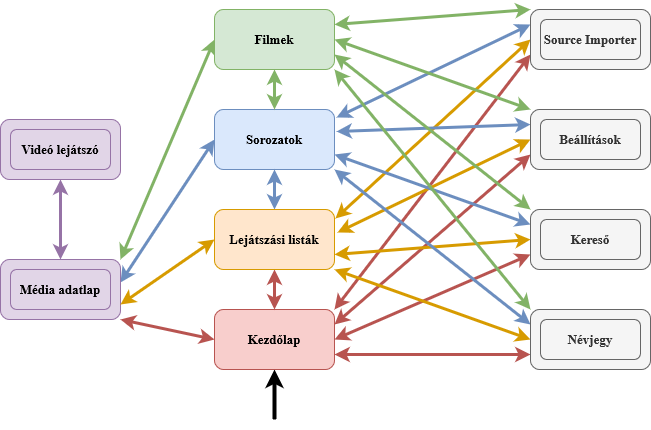
\includegraphics[width=1\textwidth]{navigation_between_screens.png}
	\caption{Navigáció az oldalak között}
	\label{fig:search}
\end{figure}

\subsection{Használati esetek diagram}
\begin{figure}[H]
	\centering
	
\includegraphics[width=1\textwidth]{use_case_diagram.jpg}
	\caption{Használati esetek diagram}
	\label{fig:use_case}
\end{figure}

% ==========================================================
% |                    Implementáció                       |
% ==========================================================
\section{Implementáció}
TODO

\subsection{Funkcionális megközelítés}
TODO

\section{Tesztelés}
TODO
